\section{Il metodo}
Per confrontare i due algoritmi procedendo in modo sperimentale, si è implementato un software che producesse
un'istanza per il problema per poi essere eseguita su entrambi gli algoritmi e produrre un grafico al fine di 
analizzare i risultati dati. 

\subsection{Generazione degli oggetti e dei bins}
Come prima cosa, dopo aver fissato il numero $ n $ di oggetti e il numero $ m $ di bins, è stato necessario generare le rispettive taglie
in base a qualche criterio in modo che rispettassero le condizioni del problema, ovvero che la somma delle taglie degli oggetti 
deve essere uguale alla somma delle taglie dei bins.

\subsubsection{Una prima soluzione}
La prima soluzione sviluppata per fare in modo che gli oggetti e i bins generati rispettassero le condizioni del problema
è stata quella di scegliere la taglia degli $ m $ bins uguale a $ 1/m $ in modo che la loro somma sia pari a $ 1 $, mentre
per gli oggetti si è proceduto nel seguente modo:
\begin{quote}
	\begin{enumerate}
		\item Si generano $ n $ numeri $ x_i \: \forall i \in \{1, ..., n\} $ in modo che ogni numero sia preso con probabilità 
			  uniforme in un intervallo di interi $ [1, M] $.
		\item Ogni oggetto $ o_i $ avrà taglia pari a $ \displaystyle\frac{x_i}{\sum_{j=1}^n x_j} \: \forall i \in \{1, ..., n\} $.
	\end{enumerate}
\end{quote}
Ovvero si è fatto in modo che la somma degli oggetti fosse normalizzata ad $ 1 $.

\paragraph{I problemi di questa soluzione}\mbox{}\\
Nonostante questo criterio di generazione sembri essere buono ai fini degli esperimenti esso comporta dei problemi una volta
realizzato su calcolatore, in quanto così facendo le taglie degli oggetti assumono valori molto piccoli, valori che non vengono
sentiti nella somma tra le varie taglie, e di conseguenza falsano i risultati. Non è possibile fare un confronto tra i due algoritmi
in quanto non effettuano le operazioni nello stesso ordine, un numero potrebbe essere sommato prima o dopo ad un altro in base all'
algoritmo eseguito, e quindi potrebbe amplificare o meno errori di calcolo, inoltre i numeri generati con questo metodo sono
anche soggetti ad arrotondamenti e troncamenti vari al crescere di $ n $ e quindi si perde precisione.


\subsubsection{Una seconda soluzione}
Visti i problemi della prima soluzione illustrata si è cercato di ridurre gli errori dovuti a numeri troppo piccoli adoperando
una tecnica diversa per la generazione degli oggetti ma simile alla prima, ovvero anziché normalizzare ad $ 1 $ la somma dei bins 
e quella degli oggetti si è preferito dare una capacità intera fissata ai bins uguale per tutti e generare le taglie degli oggetti nel
seguente modo:
\begin{quote}
	\begin{enumerate}
		\item Si generano $ n $ numeri $ x_i \: \forall i \in \{1, ..., n\} $ in modo che ogni numero sia preso con probabilità 
			  uniforme in un intervallo di interi $ [1, M] $.
		\item Ogni oggetto $ o_i $ avrà taglia pari a $ \displaystyle\frac{x_i}{\sum_{j=1}^n x_j}cm \: \forall i \in \{1, ..., n\} $. 
	\end{enumerate}
\end{quote}
Ovvero si è fatto in modo che la somma degli oggetti fosse normalizzata a $ cm $ dove $ c $ è la capacità fissata
di ogni bin e $ m $ il numero di bins.

\paragraph{I problemi di questa soluzione}\mbox{}\\
Nonostante in questo caso si lavori con numeri più grandi anche questa soluzione comporta problemi relativi
alle operazioni effettuate tramite calcolatore con valori "problematici" e di conseguenza anche questa tecnica falsa i risultati e non è possibile confrontare
i risultati degli algoritmi.


\subsubsection{Una terza soluzione}
Al fine di eliminare totalmente errori dovuti a calcoli effettuati con numeri non sentiti nella somma su calcolatore 
si è cercato di trovare un modo di generare le taglie degli oggetti e dei bins per far sì che fossero solo interi, ovvero, una volta fissati 
$ n $ ed $ m $:
\begin{quote}
	\begin{enumerate}
		\item Si generano $ n $ numeri $ o_i \: \forall i \in \{1, ..., n\} $ in modo che ogni numero sia preso con probabilità
			  uniforme in un intervallo di interi $ [1, M] $.\\
			  Sia $ sumobj $ la somma delle taglie degli oggetti.
		\item Se $ sumobj $  non è un multiplo di $ m $ allora si calcola il resto 
			  della divisione tra $ sumobj $ ed $ m $ e lo si aggiunge alla taglia di un oggetto scelto a caso, se invece è un multiplo 
			  si esegue il prossimo passo direttamente.
		\item La taglia dei bins diventa $ sumobj/m $.
	\end{enumerate}
\end{quote}
In questo modo si lavora solo con numeri interi e gli errori dovuti a numeri non sentiti nella somma con altri sono totalmente
eliminati, di conseguenza i dati sono corretti ed è possibile confrontare gli algoritmi.

\paragraph{I problemi di questa soluzione}\mbox{}\\
Anche se sono stati eliminati del tutto gli errori sui calcoli sorge un altro problema, ovvero quello dell'overflow, infatti se le taglie
degli oggetti sono troppo grandi, o comunque al crescere di $ n $, la somma di questi potrebbe provocare un'overflow. Questi problemi sono
presenti anche nelle due soluzioni precedenti al crescere di $ n $, anzi le due precedenti potrebbero portare anche ad underflow, ma ciò è trascurabile per
la riuscita dell'esperimento in quanto non è una cosa che può essere risolta in generale sotto queste condizioni.


\subsubsection{La strategia utilizzata}
Si è scelto di utilizzare l'ultima soluzione descritta per generare gli oggetti e i bins in quanto non presenta nessun problema ai fini
dell'esperimento e produce dati corretti, per cui è possibile confrontare i risultati degli algoritmi.


\subsection{Raccolta dati}
Per la parte di raccolta dati semplicemente si è definito un numero di esperimenti da eseguire e salvato i valori prodotti dagli algoritmi corrispondenti
alle istanze generate dal metodo illustrato precedentemente basato sul numero di oggetti e bins relativi all'esperimento. Una volta prodotti questi dati
essi sono stati riportati in una tabella che mette in corrispondenza i valori delle istanze e degli algoritmi eseguiti su di esse.


\subsection{Analisi grafica}
Una volta prodotti i dati dell'esperimento, al fine di renderne più facile e immediata l'analisi, essi sono stati riportati su un piano tridimensionale 
dove sull'asse delle $ x $ si trova il numero di oggetti da immagazzinare, sull'asse delle $ y $ il numero di bins, e sull'asse delle $ z $
il risultato degli algoritmi. In questo modo è immediato confrontare i valori delle esecuzioni su una stessa istanza.


\section{Aspetti tecnici dell'implementazione}
Per realizzare il software desiderato sono state fatte scelte precise riguardo le tecnologie da utilizzare spiegate di seguito.

\subsection{Linguaggio e librerie utilizzate}
Il linguaggio utilizzato per la realizzazione del software è \textit{Python}, le motivazioni di tale scelta sono da cercare nella semplicità di scrittura 
del codice data dall'alto livello di astrazione e dalla presenza di numerose librerie a supporto dell'utilizzo scientifico del linguaggio. Inoltre
non ci sono particolari caratteristiche dell'esperimento che avrebbero prediletto altri linguaggi, ad esempio se si avesse dovuto utilizzare la concorrenza 
si sarebbe optato per un linguaggio come \textit{Rust} o uno puramente funzionale come \textit{Haskell}, se il tempo di esecuzione fosse stato cruciale si sarebbe
optato per un linguaggio a basso livello come \textit{C}, ma poiché non c'è da preoccuparsi di queste questioni \textit{Python} va più che bene per lo
scopo.\\
Le librerie utilizzate all'interno del software sono:

\paragraph{heapq}\mbox{}\\
Una libreria nativa del linguaggio che permette di utilizzare una lista come uno heap ed eseguire i classici algoritmi relativi ad esso sulla lista in 
modo efficiente.\\
Usata per sfruttare il costo computazionale ridotto di uno heap per determinate operazioni al fine di ottimizzare gli algoritmi che ne fanno uso.

\paragraph{matplotlib}\mbox{}\\
Una libreria di plotting per Python orientata agli oggetti, che permette di creare grafici di ogni tipo e visualizzarli interattivamente, esponendo una API molto simile a quella del 
linguaggio \textit{Matlab}.\\
Usata all'interno del software sviluppato per creare le tabelle e i grafici relativi agli esperimenti, in particolare si sono utilizzati i moduli \texttt{pyplot} 
e \texttt{Axes3D} da \texttt{mpl\_toolkits.mplot3d}.

\paragraph{numpy}\mbox{}\\
Libreria di supporto al calcolo scientifico per il linguaggio, che espone numerose funzioni matematiche di alto livello al fine di poterle utilizzare in modo
efficiente, utilizzata anche all'interno di \texttt{matplotlib} per operare efficientemente con matrici e vettori di grandi dimensioni.\\
Usata nel software per creare liste di numeri generati casualmente tramite distribuzione uniforme, infatti si è utilizzato in particolare il modulo
\texttt{random}.

\subsection{Codice}
Per la consultazione del codice si rimanda alla \hyperref[sec:Codice]{\underline{sezione dedicata}} nell'appendice.


\section{Dati sperimentali e interpretazione}
Una volta delineato il metodo da utilizzare per l'esperimento e realizzato il software che permette di eseguirlo sono stati prodotti i dati relativi ad esso
per essere analizzati.

\subsection{Dati}
Di seguito varie immagini raffiguranti gli esiti degli esperimenti basati su istanze generate casualmente con distribuzione uniforme negli intervalli specificati.
\begin{figure}[H]
	\caption{9 esperimenti con $ n $ = $ 10m $ in $ [1, 1000] $ }
	\label{sec:Exp1}
	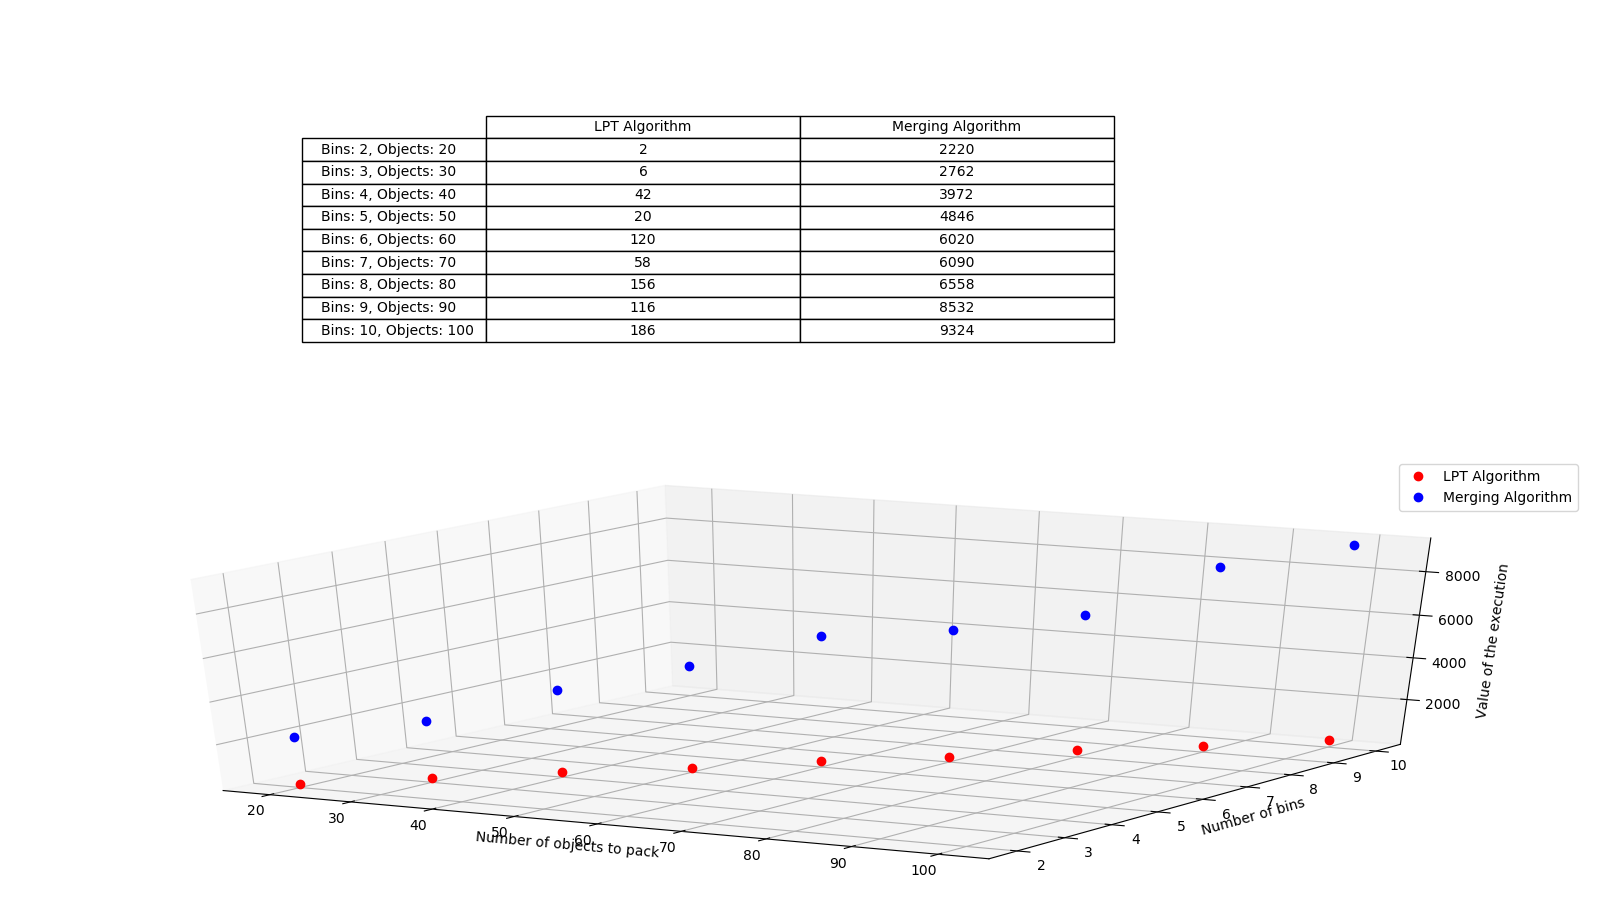
\includegraphics[scale=0.5, angle=90]{9_exps_1-1000_per10}
\end{figure}
\begin{figure}[H]
	\caption{9 esperimenti con $ n $ = $ 100m $ in $ [1, 1000] $ }
	\label{sec:Exp2}
	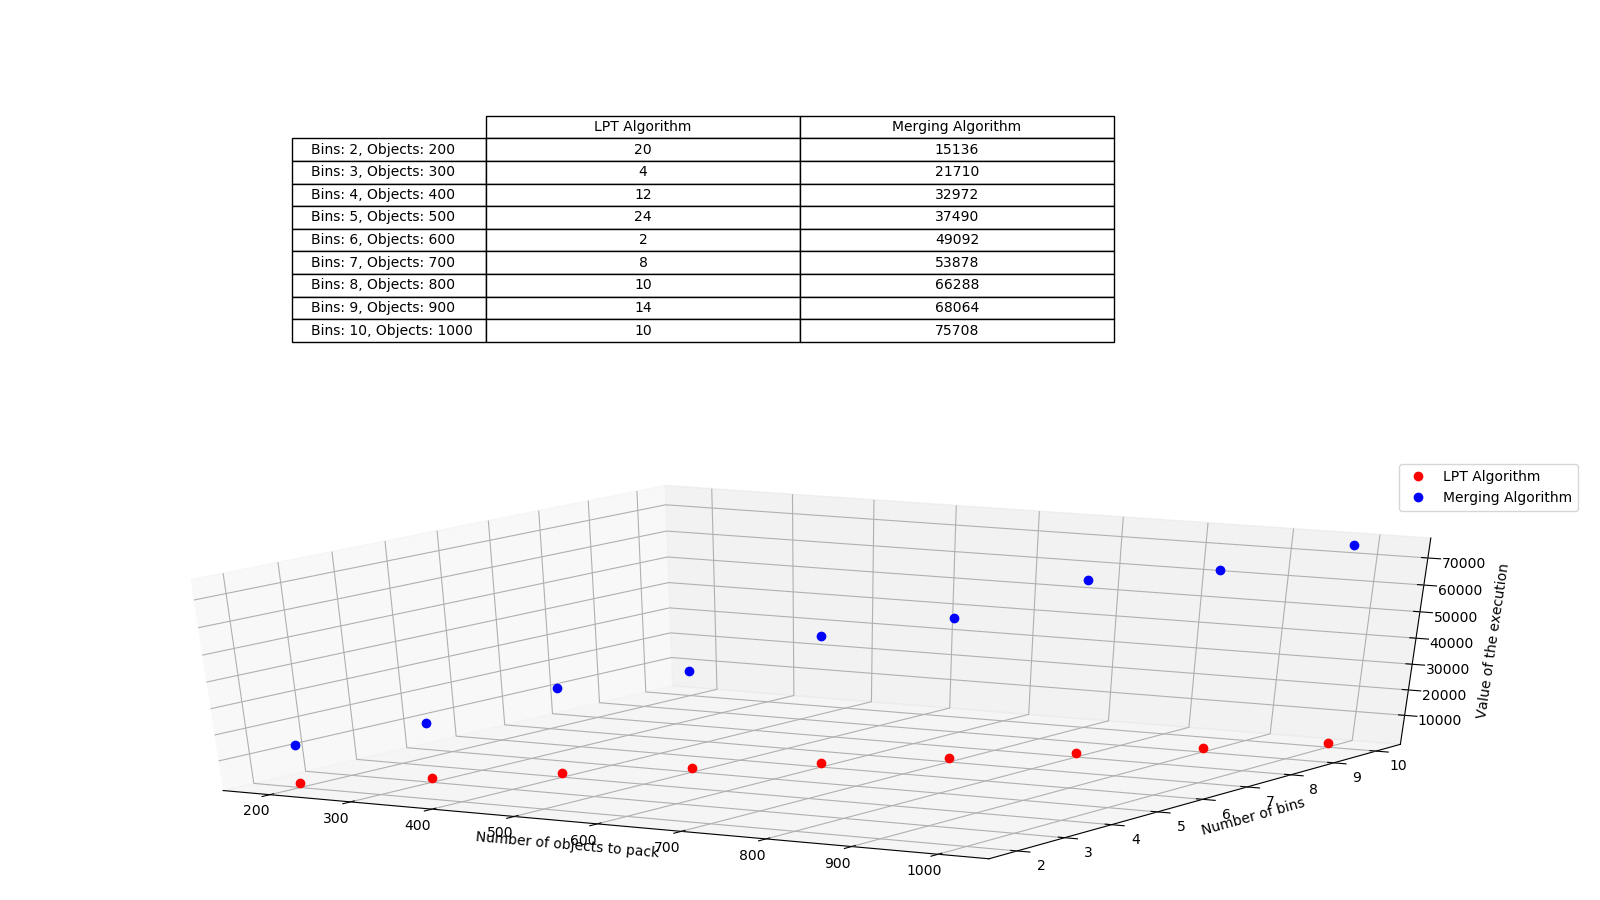
\includegraphics[scale=0.5, angle=90]{9_exps_1-1000_per100}
\end{figure}
\begin{figure}[H]
	\caption{Altri 9 esperimenti con $ n $ = $ 100m $ in $ [1, 1000] $ }
	\label{sec:Exp2.2}
	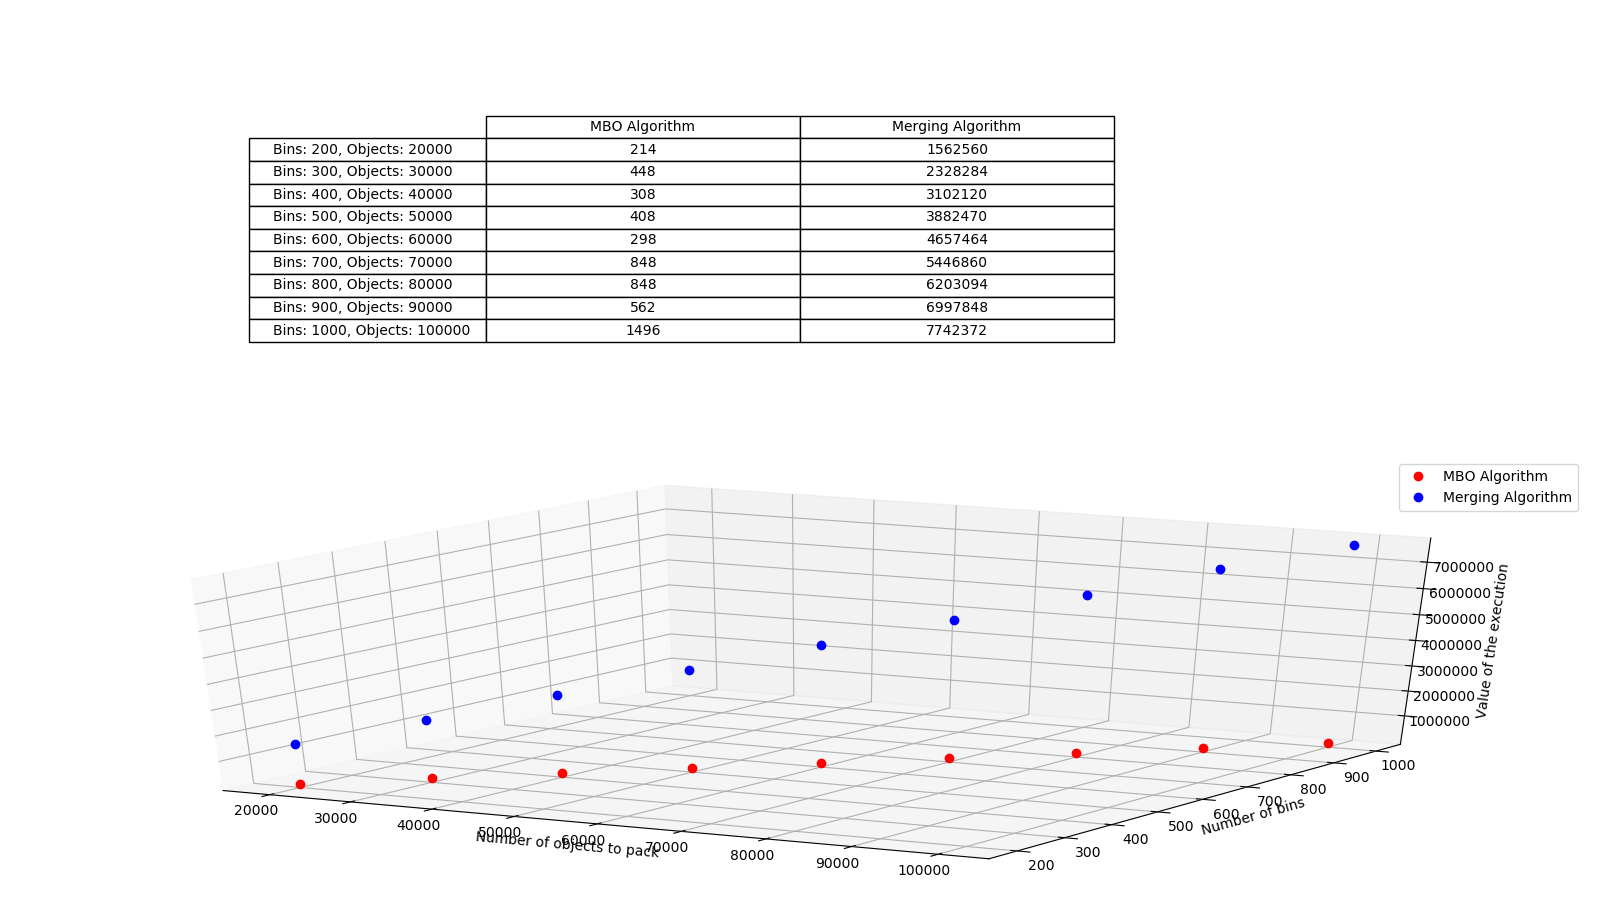
\includegraphics[scale=0.45, angle=90]{9_exps_1-1000_per100_2}
\end{figure}
\begin{figure}[H]
	\caption{9 esperimenti con $ n $ = $ 1000m $ in $ [1, 1000] $ }
	\label{sec:Exp3}
	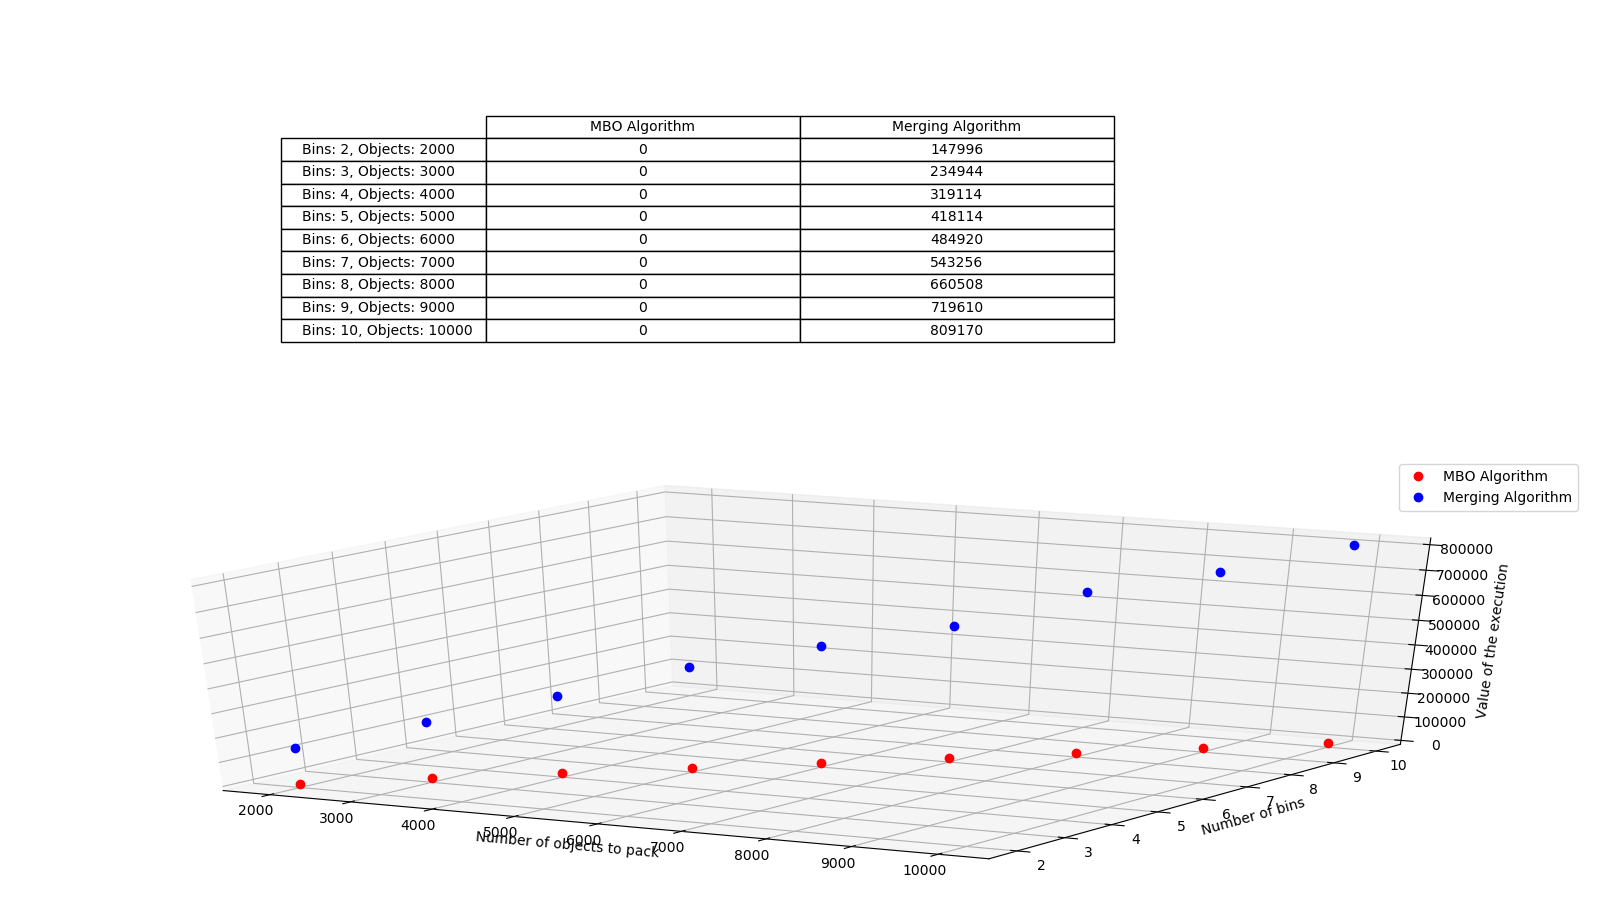
\includegraphics[scale=0.5, angle=90]{9_exps_1-1000_per1000}
\end{figure}
\begin{figure}[H]
	\caption{Altri 9 esperimenti con $ n $ = $ 1000m $ in $ [1, 1000] $ }
	\label{sec:Exp3.2}
	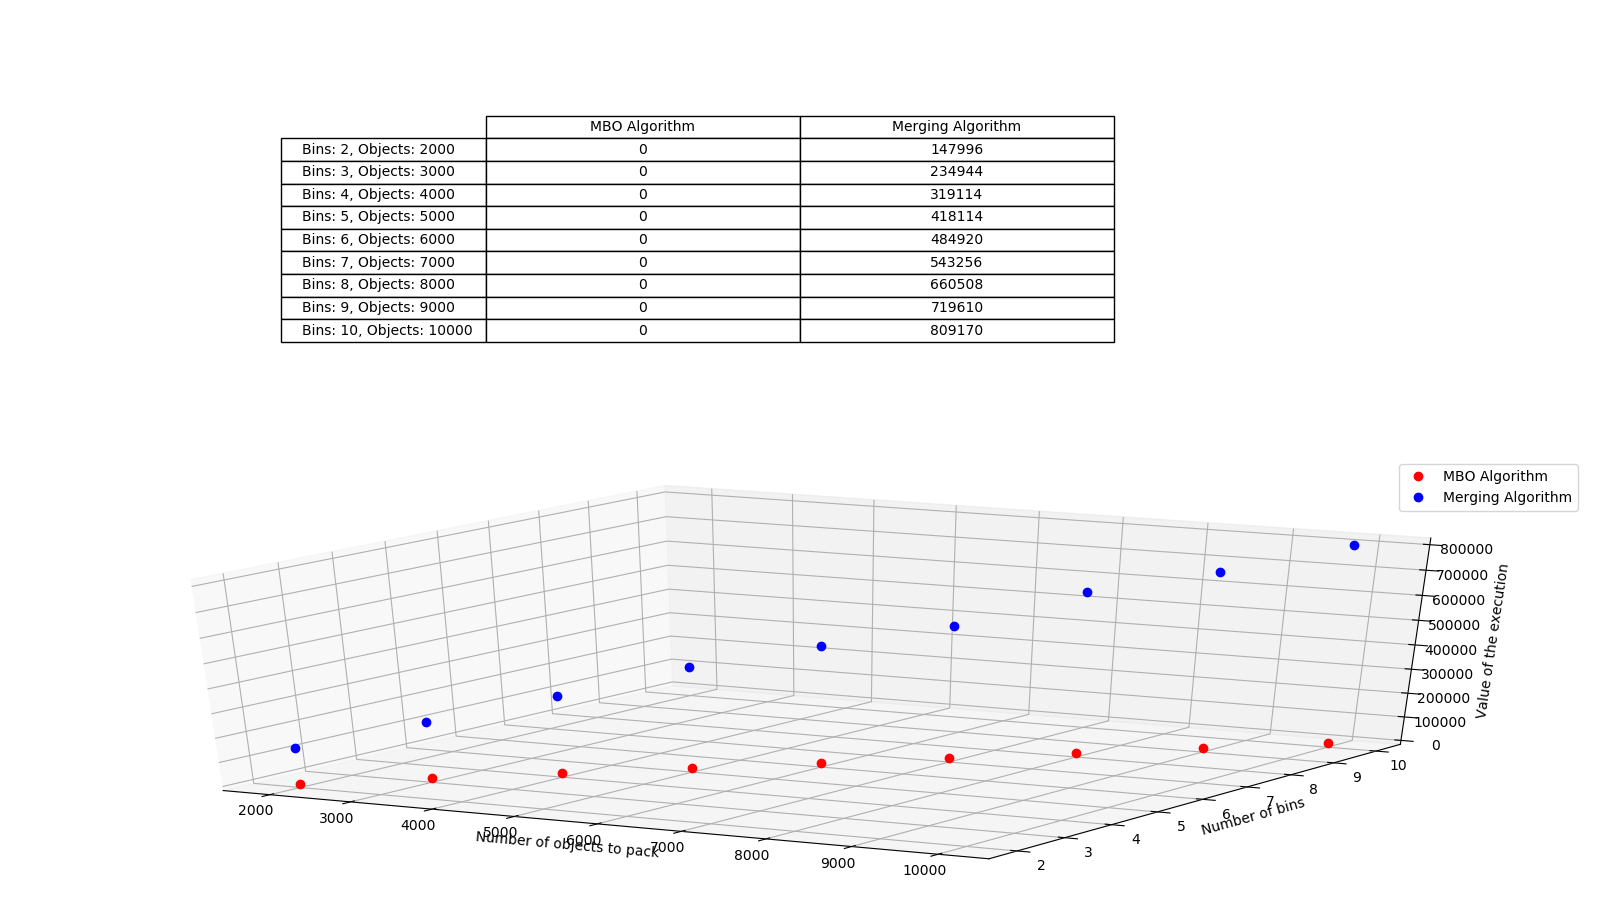
\includegraphics[scale=0.5, angle=90]{9_exps_1-1000_per1000}
\end{figure}
\begin{figure}[H]
	\caption{5 esperimenti con $ n $ = $ 10m $ progressivamente in $ [1, 1000] $ }
	\label{sec:Exp4}
	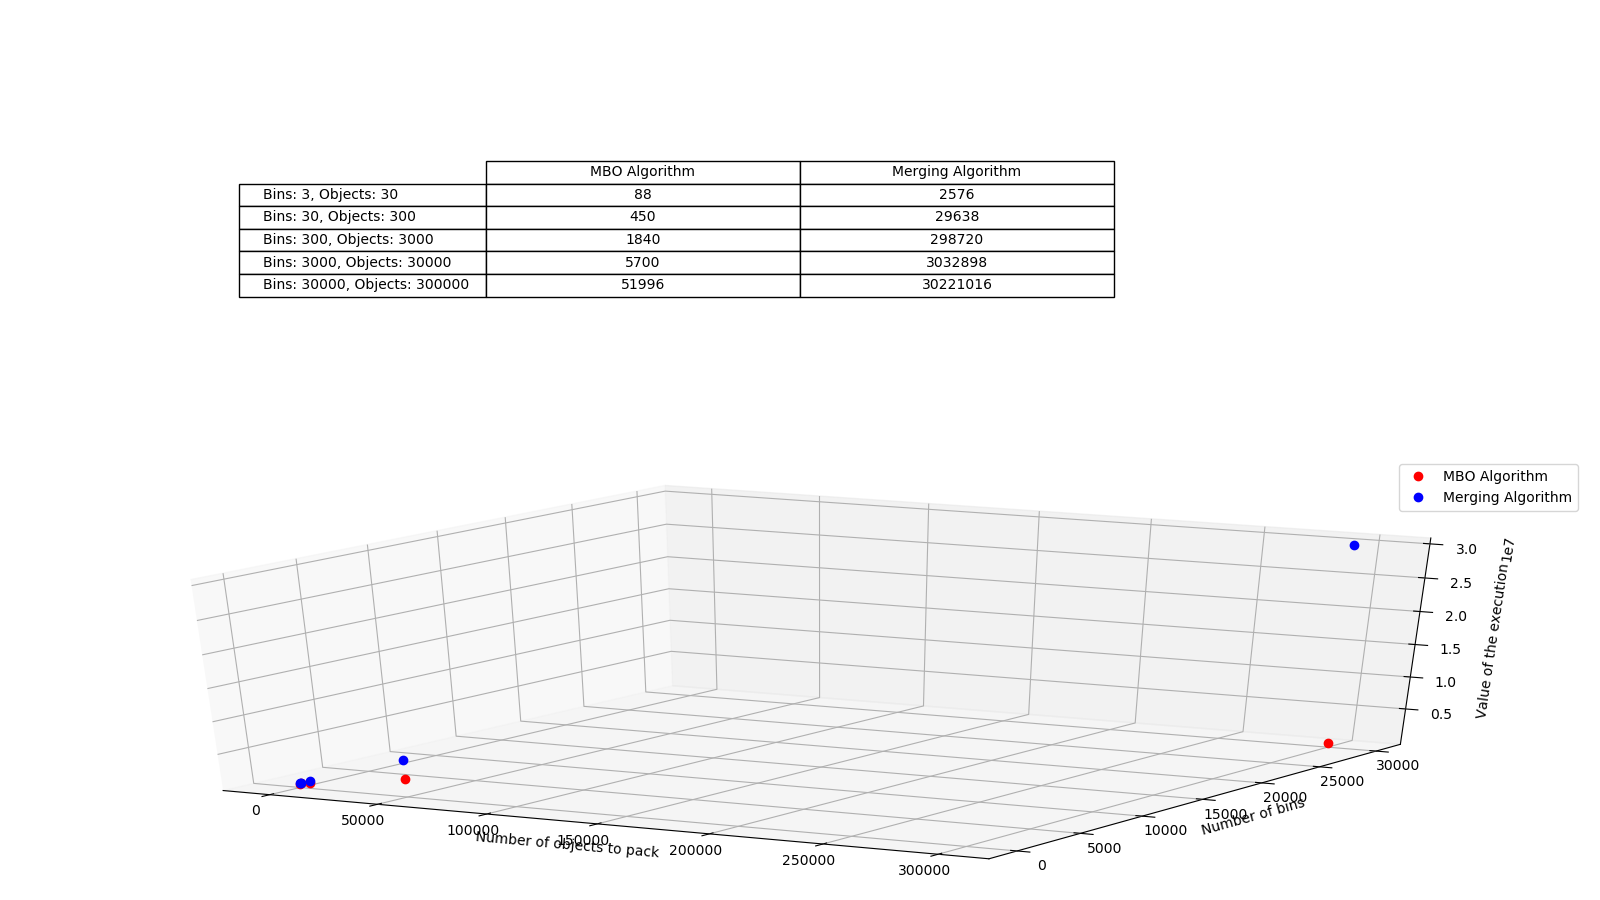
\includegraphics[scale=0.5, angle=90]{5_exps_1-1000_progressive}
\end{figure}
\begin{figure}[H]
	\caption{9 esperimenti con $ n $ = $ 1000m $ in $ [1, 10000] $ }
	\label{sec:Exp5}
	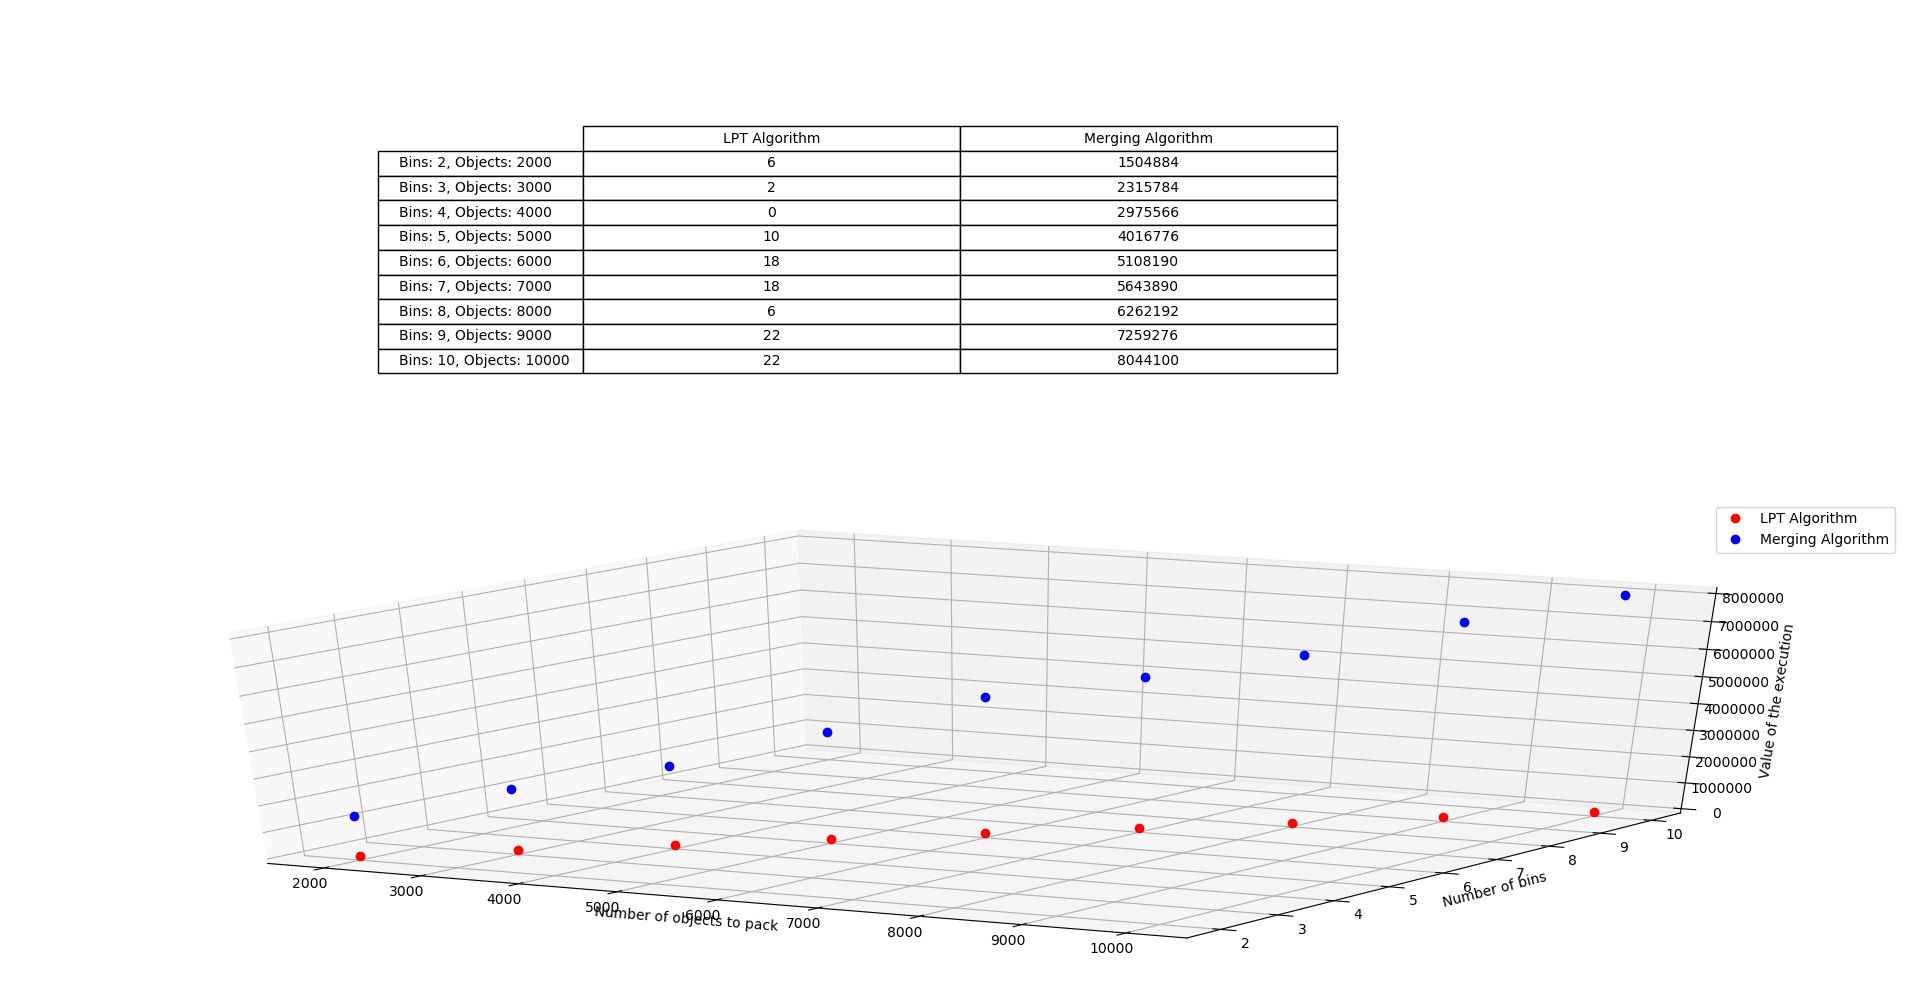
\includegraphics[scale=0.45, angle=90]{9_exps_1-10000_per1000}
\end{figure}
\begin{figure}[H]
	\caption{9 esperimenti con $ n $ = $ 1000m $ in $ [1, 100000] $ }
	\label{sec:Exp6}
	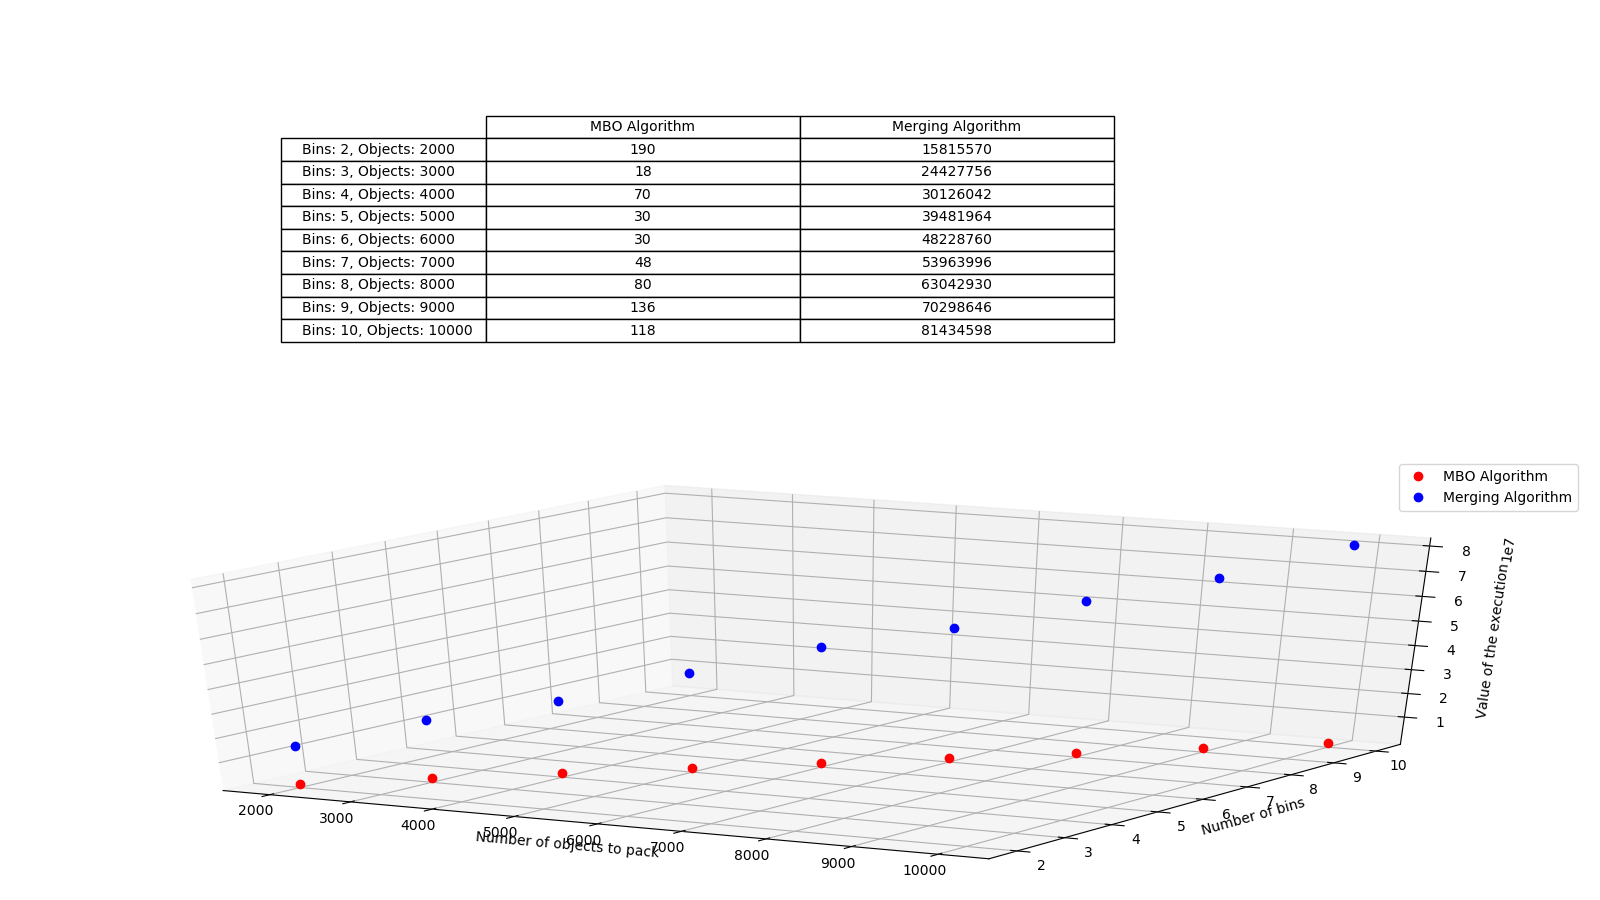
\includegraphics[scale=0.5, angle=90]{9_exps_1-100000_per1000}
\end{figure}

\subsection{Interpretazione}
Ciò che si nota a primo impatto dai risultati degli esperimenti è che l'algoritmo con euristica LPT, su istanze generate in modo casuale, dà sempre un risultato
di gran lunga migliore rispetto all'algoritmo con euristica di merging sugli oggetti in ogni caso.\\
È possibile notare come al crescere del numero di oggetti rispetto al numero di bins, fissato l'intervallo di generazione, l'algoritmo LPT migliora sempre la 
propria soluzione (visibile analizzando questi esperimenti: \hyperref[sec:Exp1]{\underline{Figura 1}}, \hyperref[sec:Exp2]{\underline{Figura 2}}, 
\hyperref[sec:Exp3]{\underline{Figura 3}}) arrivando addirittura a disporli perfettamente all'interno dei contenitori senza il minimo spreco o eccesso di spazio. Al
contrario l'algoritmo di merging ha un comportamento opposto, ovvero peggiora sempre la propria soluzione.\\
Inoltre si nota come prendendo un intervallo più grande di generazione (\hyperref[sec:Exp5]{\underline{Figura 5}}, \hyperref[sec:Exp6]{\underline{Figura 6}}) 
l'algoritmo LPT non dispone sempre perfettamente gli oggetti nei contenitori ma dà comunque risultati migliori rispetto a quello di merging.


\section{Conclusioni}
Dopo aver effettuato i vari esperimenti ed analizzato i dati si può concludere dicendo che in generale, se gli oggetti hanno taglie "varie" e quindi l'istanza del problema
non ha una particolare forma, l'algoritmo LPT dà risultati migliori rispetto a quello di merging. Quindi poiché la complessità temporale asintotica è praticamente
la stessa si può affermare che conviene utilizzare il primo algoritmo menzionato in quanto ci darà una soluzione nettamente migliore rispetto al secondo.\\
È comunque da tenere in considerazione la natura dell'istanza, in quanto ce ne potrebbero essere alcune per cui gli algoritmi danno la stessa soluzione, oppure per cui la
"distanza" tra le due soluzioni non sia così grande come si vede dagli esperimenti, o che addirittura, come visto in precedenza, producano quella ottima.